\documentclass[a4paper,11pt,notitlepage]{article}
\usepackage[utf8]{inputenc}
\usepackage[T1]{fontenc}
\usepackage[polish]{babel}
\usepackage[MeX]{polski}
\selectlanguage{polish}
\usepackage[top=2cm, bottom=2cm, left=2cm, right=2cm]{geometry}
\usepackage{listings}
\usepackage{graphicx}

\author{ Michał Zochniak }
\title{ Testowanie }

\date{\today}
\begin{document}
\maketitle

\section{Testy czarnoskrzynkowe interpolacji}

\subsection{Testy interpolacji w węzłach}

\subsubsection{Opis}

Została napisana klasa testowa za pomocą JUnit służąca do testowania własności $S(x_i) = f(x_i)$ gdzie $S$ to funkcja interpolująca, $f$ to funkcja wzorcowa a $x_i$ to zadany węzęł.

\subsubsection{Sposób realizacji}

Klasa testowa jest zbudowana przy pomocy testu parametryzowanego. Zostają zadane różne zestawy danych testowych, składających się z funkcji wzorcowej postaci: tablice double x zawierająca węzły oraz tablica double y zawierająca wartości funkcji wzorcowej w węzłach. Następnie dla każdego zestawu sprawdzane jest, czy wynik interpolacji w węźle $x[i]$ jest równy wartości funkcji wzorcowej $y[i]$

\begin{lstlisting}
class KnotTestParameter
{
    public KnotTestParameter(double[] x, double[] y)
    {
        this.x = x;
        this.y = y;
    }

    public double[] x;
    public double[] y;
}

@RunWith(value = Parameterized.class)
public class KnotTest
{
    KnotTestParameter param;

    public KnotTest(KnotTestParameter param)
    {
        this.param = param;
    }

    @Parameters
    public static Collection<Object[]> params()
    {
       	/* ... */
    }

    @Test
    public void testKnot()
    {
        CubicSplineFast spline = new CubicSplineFast(param.x, param.y);
        for(int i = 0; i < param.x.length; i++)
        {
            assertEquals(param.y[i], spline.interpolate(param.x[i]), EPS);
        }
    }

}
\end{lstlisting}

Oczekujemy tego, że w węzłach wartości funkcji interpolującej będą takie same jak wartości funkcji wzorcowej. Trzeba wziąć pod uwagę ewentualne błędy precyzji/zaokrągleń.

\subsubsection{Wynik}

klasa failuje (nieraz)

\subsection{Testy interpolacji z wyrocznią}

\subsubsection{Opis}

Klasa została przetestowana pod kątem zgodności z inną implementacją interpolacji za pomocą funkcji sklejanych. Jako wyrocznia został wybrany program \textbf{Matlab 7.12.0}.

\subsubsection{Sposób realizacji}

Została stworzona klasa w Javie do generowania danych do Matlaba. Klasa dostaje funkcję wzorcową (węzły oraz wartości węzłów) oraz argumenty dla których ma być dokonana interpolacja. Następnie dokonywana jest interpolacja dla tych argumentów a jej wynik zapisywany. Tworzony jest zestaw danych do Matlaba:

\begin{lstlisting}
knownX = [-2.0, ... 2.0]; % wezly
knownY = [-0.9092, ... 0.9092]; % wartosci funkcji w wezlach
intX = [-0.5, ... -0.2]; % argumenty do interpolacji
intY = [-0.4794, ... 0.3894]; % wyniki interpolacji CubicSplineFast
\end{lstlisting}

Następnie dla danych testowych wywoływany jest skrypt w Matlabie który dokonuje interpolacji za pomocą funkcji spline. Następnie interpolacja Matlabem jest porównywana do interpolacji CubicSplineFast. Sprawdzana jest również monotoniczność otrzymanej funkcji.

\begin{lstlisting}
matlabY = spline(knownX, knownY, intX);
diff = intY - matlabY;
disp(['Largest error: ' num2str(max(abs(diff)))]);
for i = 2:length(intX)
    diffInt = intY(i) - intY(i-1);
    diffMat = matlabY(i) - matlabY(i-1);
    if(sign(diffInt) ~= sign(diffMat))
        disp(['Monotony fail: ' num2str(i) ' int: ' num2str(diffInt) ' matlab: ' num2str(diffMat)])
    end
end
\end{lstlisting}

Oczekujemy tego, że wyniki interpolacji będą mniej lub bardziej się pokrywać i będą miały taki sam kształt. Trzeba wziąć pod uwagę błędy precyzji oraz to, że Matlab prawdopodobnie implementuje inny (lepszy?) algorytm interpolacji funkcjami sklejanymi.

\subsubsection{Wynik}

We wszystkich przypadkach testowych obserwujemy mniejsze lub większe odchylenia interpolacji Matlabowej od interpolacji CubicSplineFast. Każdy testowany przypadek przeszedł ``test monotoniczności'' czyli można uznać że otrzymywane krzywe miały taki sam kształt.

Wykonane zostały testy na następujących funkcjach:

Funkcja $f(x) = 5$

Węzły $x = [0:1:10]$

Interpolowana w punktach $x = [0:0.01:10]$

Wynik klasy pokrywa się (nie licząc błędów precyzji rzędu $10^{-16}$) z wynikiem otrzymanym w Matlabie.

Funkcja fajna

%	3 & x = 0
%	8 & x = 1
%	7 & x = 2
%	8 & x = 3
%	5 & x = 4
%	3 & x = 5
%	5 & x = 6
%	5 & x = 7
%	6 & x = 8
%	1 & x = 9
%	3 & x = 10

Interpolowana w punktach $x = [0:0.01:10]$

Wyniki interpolacji:\\
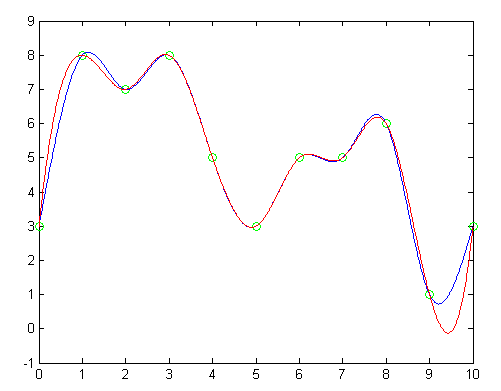
\includegraphics{spline2.png}
Zielony: funkcje wzorcowe
Czerwony: funkcja interpolująca z Matlaba
Niebieski: funkcja interpolująca z CubicSplineFast

Wynik interpolacji w Matlabie nie pokrywa się z interpolacją klasy. Różne kształty krzywych. Obie interpolacje spełniają warunek $S(x_i) = f(x_i)$.

Funkcja $f(x) = sin(x)$

Węzły $x = [-5:0.7:5]$

Interpolowana w punktach $x = [-3:0.05:3]$

Wykres różnic:\\
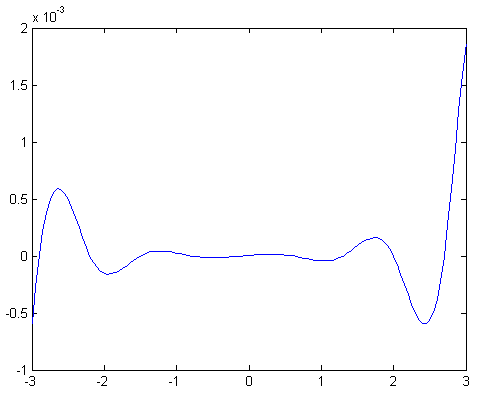
\includegraphics{spline3.png}

Wyniki interpolacji są zbliżone (największa różnica $0.0018616$, punkty przegięcia takie same). Największe różnice są na krańcach przedziałów.

Funkcja $f(x) = x^3 + x^2$

Węzły $x = [-3:0.1:5]$

Interpolowana w punktach $x = [-3:0.05:5]$

Wykres różnic:\\
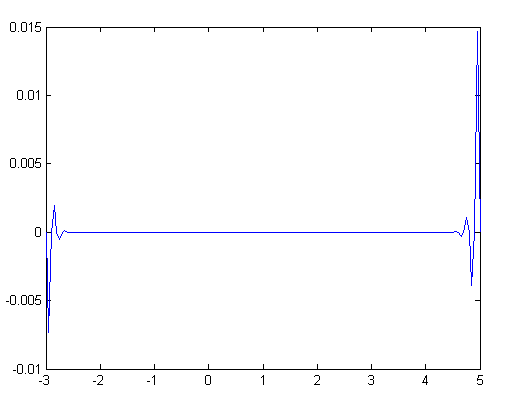
\includegraphics{spline4.png}

Wyniki interpolacji są zbliżone (największa różnica $0.014641$, punkty przegięcia takie same). Największe różnice są na krańcach przedziałów.

Funkcja $f(x) = x^-3$

Węzły $x = [2:1:2] \ 0$

Interpolowana w punktach $x = [-0.5:0.01:0.5]$

Wykres różnic:\\
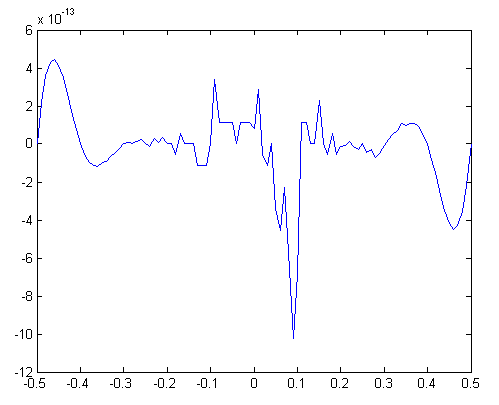
\includegraphics{spline5.png}

Wyniki interpolacji są zbliżone (największa róznica $1.0232 * 10^{-12}$, punkty przegięcia takie same).

\end{document}